\documentclass[11pt]{amsart}
\usepackage[margin=1.15in]{geometry}
\usepackage{amssymb,amsmath,mathtools}
\usepackage{graphicx,float}
\usepackage[hidelinks]{hyperref}
\usepackage[expansion=false]{microtype}

\newtheorem{theorem}{Theorem}[section]
\newtheorem{proposition}[theorem]{Proposition}
\newtheorem{lemma}[theorem]{Lemma}
\newtheorem{corollary}[theorem]{Corollary}
\newtheorem{mainthm}{Theorem}
\renewcommand{\themainthm}{\Alph{mainthm}}
\newtheorem{maincor}[mainthm]{Corollary}
\theoremstyle{definition}
\newtheorem{definition}[theorem]{Definition}
\newtheorem{remark}[theorem]{Remark}
\newtheorem{example}[theorem]{Example}
\newtheorem*{question}{Question}

\newcommand{\RR}{\mathbb{R}}
\newcommand{\CC}{\mathbb{C}}
\newcommand{\QQ}{\mathbb{Q}}
\newcommand{\NN}{\mathbb{N}}
\DeclareMathOperator{\ML}{ML}
\DeclareMathOperator{\LND}{LND}
\DeclareMathOperator{\Aut}{Aut}
\DeclareMathOperator{\Frac}{Frac}
\DeclareMathOperator{\trdeg}{tr.deg}
\newcommand{\MLs}{\ML^{*}}
\newcommand{\LNDs}{\LND^{*}}
\newcommand{\td}[1]{\trdeg_k #1}
\newcommand{\zenodoCodeDOI}{10.5281/zenodo.24123917}

\setlength{\emergencystretch}{2.5em}
\hbadness=2000
\raggedbottom
\begin{document}

\title[The Makar-Limanov invariant equals its slice version]{The Makar-Limanov Invariant Equals\\ Its Slice Version in Dimension Three}

\author{Deep Bhattacharjee}
\address{Formerly, Electro-Gravitational Space Propulsion Laboratory (EGSPL), Bhubaneswar, Odisha 751030, India}
\address{Formerly, University of Calcutta (Heramba Chandra College), 23/49 Gariahat Road, Golpark, Kolkata 700029, West Bengal, India}
\email{d.bhattacharjee@erl-forschung.de}
\email{itsdeep@live.com}
\email{egspl@proton.me (GitHub-related contact; GitHub account creelie)}
\urladdr{https://orcid.org/0000-0003-0466-750X}

\begin{abstract}
Over any field of characteristic zero, the Makar-Limanov invariant of a domain coincides with its slice version whenever the latter has transcendence degree at most one or one less than that of the domain. In dimension three this settles a question of Dasgupta and Gupta, which had been answered only over algebraically closed fields.

\medskip\noindent\textbf{Keywords:} locally nilpotent derivation; Makar-Limanov invariant; slice.

\smallskip\noindent\textbf{MSC 2020:} 14R10 (primary); 13N15, 13A50, 14R20.
\end{abstract}

\maketitle

\section{Introduction}\label{sec:intro}

Let $k$ be a field of characteristic zero and $B$ a commutative $k$-domain. A $k$-derivation $D$ of $B$ is \emph{locally nilpotent} if every element of $B$ is killed by some power of $D$; the set of these derivations is written $\LND(B)$. Makar-Limanov introduced the ring
\[
\ML(B)=\bigcap_{D\in\LND(B)}\ker D
\]
to prove that the Koras--Russell threefold $x+x^2y+z^2+t^3=0$ is not isomorphic to $\CC^3$ although it is contractible \cite{ML96}. Since then $\ML$ has been one of the main tools of affine algebraic geometry. Gupta used a characteristic-free version of it, built from exponential maps, to show that the Zariski cancellation problem has a negative answer for the affine three-space in positive characteristic \cite{Gup14a,Gup14b}. The invariant has a known weakness: it can become trivial after adding a variable. Dubouloz proved that the cylinder over the Koras--Russell threefold has trivial Makar-Limanov invariant, the same as the affine four-space \cite{Dub09}.

Freudenburg introduced a variant that only uses derivations with a slice \cite{Fre17}. An element $s\in B$ is a \emph{slice} of $D\in\LND(B)$ if $D(s)=1$. Let $\LNDs(B)$ be the set of locally nilpotent derivations of $B$ that have a slice, and put
\[
\MLs(B)=\bigcap_{D\in\LNDs(B)}\ker D,\qquad\text{with }\MLs(B)=B\text{ if }\LNDs(B)=\emptyset .
\]
If $\LNDs(B)\neq\emptyset$, the intersection defining $\ML(B)$ runs over more derivations, so $\ML(B)\subseteq\MLs(B)$; if $\LNDs(B)=\emptyset$ the inclusion holds trivially. Dasgupta and Gupta used both rings to characterise the affine plane and the affine three-space \cite{DG21}. Their main theorem says that, for a three-dimensional affine UFD $B$ over an algebraically closed field of characteristic zero, the following are equivalent: (I) $B=k^{[3]}$; (II) $\MLs(B)=k$; (III) $\ML(B)=k$ and $\MLs(B)\neq B$. They showed that the hypotheses ``algebraically closed'' and ``UFD'' cannot be dropped from (III)$\Rightarrow$(I), and they asked whether they can be dropped from (III)$\Rightarrow$(II).\footnote{The question is numbered 4.8 in the preprint version of \cite{DG21} and is cited as Question~5.9 in \cite{GS24}. We quote it verbatim.}

\begin{question}[Dasgupta--Gupta \cite{DG21}]
Does there exist a three-dimensional affine $k$-domain $B$ over a field $k$ of characteristic zero such that $\ML(B)=k$ but $\td{\MLs(B)}=1$?
\end{question}

They proved that the answer is negative when $k$ is algebraically closed and $B$ is a UFD, and observed that a negative answer in general would give (III)$\Rightarrow$(II) for every three-dimensional affine domain over every field of characteristic zero. Gaifullin and Shafarevich then proved that $\ML(B)=\MLs(B)$ whenever $\LNDs(B)\neq\emptyset$, for every affine domain over an \emph{algebraically closed} field of characteristic zero \cite[Theorem~1]{GS24}. Their proof compares orbits of the subgroups of $\Aut(B)$ generated by the corresponding unipotent one-parameter groups, through the work of Arzhantsev, Flenner, Kaliman, Kutzschebauch and Zaidenberg on flexible varieties \cite{AFKKZ13}. It needs points over $k$ in general position and so does not apply to fields such as $\RR$ or $\QQ$. Neither invariant commutes with extension of the base field (Section~\ref{sec:examples}), so the question over non-closed fields cannot be reduced to the closed case.

We answer the question over every field of characteristic zero, without any finiteness or factoriality assumption, by a short argument with no geometry in it.

\begin{mainthm}\label{thmA}
Let $k$ be a field of characteristic zero and $B$ a $k$-domain with $\td{\MLs(B)}\le 1$. Then $\ML(B)=\MLs(B)$.
\end{mainthm}

\begin{mainthm}\label{thmB}
Let $k$ be a field of characteristic zero and $B$ a $k$-domain of finite transcendence degree $n\ge1$ over $k$ with $\td{\MLs(B)}=n-1$. Then $\ML(B)=\MLs(B)=\ker E$ for every nonzero $E\in\LND(B)$, the ring $\MLs(B)$ has no nonzero locally nilpotent derivation, and $B$ is a polynomial ring in one variable over $\MLs(B)$.
\end{mainthm}

For affine domains Theorem~\ref{thmB} is a lemma of Dasgupta and Gupta \cite[Lemma~3.2]{DG21}, whose proof rests on a theorem of Crachiola and Makar-Limanov on rigid rings \cite{CML05}. The proof given here does not use that theorem, and it works for every domain of finite transcendence degree. For $\td{B}\le2$ and $\LNDs(B)\neq\emptyset$ the equality $\ML(B)=\MLs(B)$ was known over every field of characteristic zero \cite{DG21,Sai24}; Theorem~\ref{thmA} is new over fields that are not algebraically closed as soon as $\td{B}\ge3$. Together they cover every value of $\td{\MLs(B)}$ when $\td{B}\le 3$.

\begin{mainthm}\label{thmC}
Let $k$ be a field of characteristic zero and $B$ a $k$-domain with $\td{B}\le 3$ and $\LNDs(B)\neq\emptyset$. Then $\ML(B)=\MLs(B)$.
\end{mainthm}

\begin{maincor}\label{corD}
Over a field of characteristic zero there is no domain $B$ of transcendence degree three, affine or not, with $\ML(B)=k$ and $\td{\MLs(B)}=1$. More generally, if $\td{B}=n$, $\ML(B)=k$ and $k\neq\MLs(B)\neq B$, then $2\le\td{\MLs(B)}\le n-2$. In particular the conditions (II) and (III) above are equivalent for every three-dimensional domain over every field of characteristic zero.
\end{maincor}

The proof rests on one observation, which has nothing to do with the dimension: $\MLs(B)$ is mapped into itself by \emph{every} locally nilpotent derivation of $B$, not only by those with a slice (Proposition~\ref{prop:stable}). The reason is that the exponential of such a derivation is an automorphism of $B$, and conjugating a derivation with a slice by an automorphism gives another derivation with a slice. Once this is known, any locally nilpotent derivation $E$ restricts to $\MLs(B)$, and if the restriction is not zero, a local slice of the restriction can be divided by its image when the kernel of the restriction is small. The quotient is a slice of $E$ itself, so $E$ kills $\MLs(B)$ after all. This works when the kernel of the restriction is algebraic over $k$, which is guaranteed by $\td{\MLs(B)}\le1$. In the case $\td{\MLs(B)}=n-1$ the ring $\MLs(B)$ is the kernel of a slice derivation, and it has no nonzero locally nilpotent derivations at all.

The remaining range $2\le\td{\MLs(B)}\le n-2$ for $n\ge4$ is open over non-closed fields; Figure~\ref{fig:ladder} shows what is settled.

\begin{figure}[H]
\centering
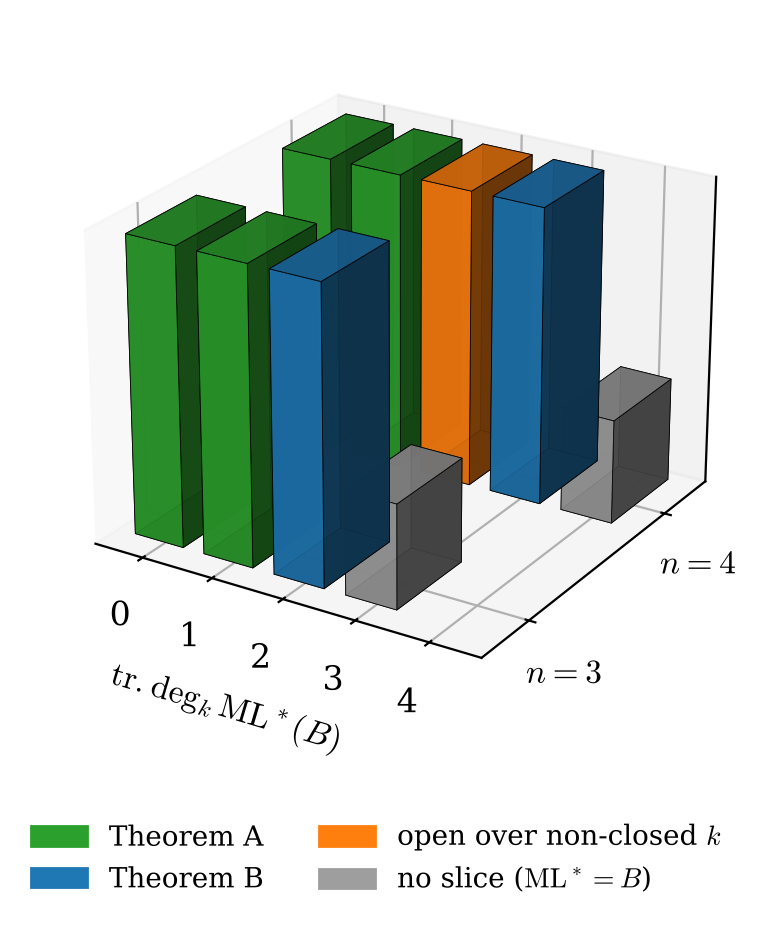
\includegraphics[width=0.52\textwidth]{fig_ladder.png}
\caption{Which values of $\td{\MLs(B)}$ are settled for $\td{B}=3$ and $\td{B}=4$ over an arbitrary field of characteristic zero. The value $\td{B}$ itself occurs exactly when $\LNDs(B)=\emptyset$, where the two rings may differ \cite{DG21}. Over algebraically closed fields every value is settled by \cite{GS24}.}
\label{fig:ladder}
\end{figure}

The paper is self-contained apart from elementary facts on transcendence degree. Section~\ref{sec:prelim} proves the facts on locally nilpotent derivations that we use, including the slice theorem. Section~\ref{sec:stable} contains the stability of $\MLs$. Section~\ref{sec:proofs} proves the theorems, and Section~\ref{sec:examples} discusses examples over the real numbers which show that the two invariants change under extension of scalars.

\medskip\noindent\textbf{Conventions.} Throughout, $k$ is a field of characteristic zero, rings are commutative with identity, and $B$ is a $k$-domain, that is, a $k$-algebra which is an integral domain. We write $\td{C}$ for the transcendence degree over $k$ of the fraction field of a $k$-domain $C$. An element $b$ of $B$ is \emph{algebraic over} a subring $C$ if $P(b)=0$ for a nonzero polynomial $P\in C[T]$; since denominators can be cleared, this is the same as being algebraic over $\Frac(C)$. A subring $C\subseteq B$ is \emph{algebraically closed in} $B$ if every element of $B$ algebraic over $C$ lies in $C$. For a ring $C$, $C^{[1]}$ denotes a polynomial ring in one variable over $C$. A domain is \emph{rigid} if it has no nonzero locally nilpotent derivation.

\section{Locally nilpotent derivations}\label{sec:prelim}

A $k$-derivation $D$ of $B$ is $k$-linear and satisfies $D(ab)=aD(b)+bD(a)$. From $D(1)=D(1\cdot1)=2D(1)$ we get $D(1)=0$, hence $D(\lambda)=0$ for $\lambda\in k$, and $\ker D$ is a $k$-subalgebra of $B$. By induction on $m$ one has the Leibniz formula
\begin{equation}\label{eq:leibniz}
D^m(ab)=\sum_{i=0}^{m}\binom{m}{i}D^i(a)\,D^{m-i}(b).
\end{equation}

\begin{lemma}\label{lem:generators}
Let $D$ be a $k$-derivation of $B$. The elements of $B$ killed by some power of $D$ form a $k$-subalgebra. In particular, if $B$ is generated as a $k$-algebra by elements each killed by a power of $D$, then $D\in\LND(B)$.
\end{lemma}

\begin{proof}
The set is closed under sums and multiplication by elements of $k$, since $D^m$ is $k$-linear and $D^m(b)=0$ implies $D^{m'}(b)=0$ for $m'\ge m$. If $D^m(a)=0$ and $D^n(b)=0$, every term of \eqref{eq:leibniz} for $D^{m+n}(ab)$ vanishes: for $i\ge m$ the factor $D^i(a)$ is zero, and for $i<m$ the factor $D^{m+n-i}(b)$ is zero because $m+n-i>n$.
\end{proof}

For $D\in\LND(B)$ and $t\in k$ put
\[
\exp(tD)(b)=\sum_{i\ge0}\frac{t^i}{i!}D^i(b),
\]
a finite sum for each $b$. Division by $i!$ is allowed because $k$ has characteristic zero.

\begin{lemma}\label{lem:exp}
For $D\in\LND(B)$ and $t,u\in k$, the map $\exp(tD)$ is a $k$-algebra endomorphism of $B$, and $\exp(tD)\circ\exp(uD)=\exp((t+u)D)$. In particular $\exp(tD)$ is an automorphism with inverse $\exp(-tD)$.
\end{lemma}

\begin{proof}
Linearity over $k$ and $\exp(tD)(1)=1$ are clear. By \eqref{eq:leibniz},
\[
\exp(tD)(ab)=\sum_{m\ge0}\frac{t^m}{m!}\sum_{i+j=m}\frac{m!}{i!\,j!}D^i(a)D^j(b)=\Bigl(\sum_{i}\frac{t^i}{i!}D^i(a)\Bigr)\Bigl(\sum_j\frac{t^j}{j!}D^j(b)\Bigr).
\]
Since $\exp(uD)(b)$ is a finite $k$-linear combination of the $D^j(b)$, all sums below are finite, and
\[
\exp(tD)\exp(uD)(b)=\sum_{i,j}\frac{t^iu^j}{i!\,j!}D^{i+j}(b)=\sum_{m}\frac{1}{m!}\Bigl(\sum_{i+j=m}\frac{m!}{i!\,j!}t^iu^j\Bigr)D^m(b)=\exp((t+u)D)(b).
\]
Taking $u=-t$ and using $\exp(0\cdot D)=\mathrm{id}$ gives the inverse.
\end{proof}

The next lemma is the place where characteristic zero enters most directly.

\begin{lemma}\label{lem:algclosed}
Let $\delta$ be a $k$-derivation of a $k$-domain $C$ and $A=\ker\delta$. Every element of $C$ algebraic over $A$ lies in $A$. In particular $\ker\delta$ is algebraically closed in $C$, and every element of $C$ algebraic over $k$ lies in $\ker\delta$.
\end{lemma}

\begin{proof}
Let $b\in C$ be algebraic over $A$, and choose a nonzero $P=\sum_{i=0}^m a_iT^i\in A[T]$ with $P(b)=0$ and $m$ as small as possible; then $m\ge1$ and $a_m\neq0$, since a nonzero constant does not vanish at $b$. Applying $\delta$ to $P(b)=0$ and using $\delta(a_i)=0$ gives
\[
0=\sum_{i=1}^m ia_ib^{i-1}\delta(b)=P'(b)\,\delta(b),\qquad P'=\sum_{i=1}^m ia_iT^{i-1}\in A[T].
\]
The leading coefficient $ma_m$ of $P'$ is nonzero because $k$ has characteristic zero and $C$ is a domain, so $P'$ is a nonzero polynomial of degree $m-1<m$. By the minimality of $m$, $P'(b)\neq0$. As $C$ is a domain, $\delta(b)=0$. The last assertion follows because $k\subseteq A$.
\end{proof}

\begin{lemma}\label{lem:localslice}
Let $\delta$ be a nonzero locally nilpotent derivation of a $k$-domain $C$ and $A=\ker\delta$. There is $g\in C$ with $c=\delta(g)\neq0$ and $\delta(c)=0$. Such an element $g$ is not algebraic over $A$. Consequently, if $\td{C}$ is finite, then $\td{A}\le\td{C}-1$.
\end{lemma}

\begin{proof}
Pick $f\in C$ with $\delta(f)\neq0$ and let $N\ge1$ be the largest integer with $\delta^N(f)\neq0$; it exists because $\delta$ is locally nilpotent. Then $g=\delta^{N-1}(f)$ has $\delta(g)=\delta^N(f)\neq0$ and $\delta^2(g)=0$. If $g$ were algebraic over $A$, Lemma~\ref{lem:algclosed} would give $\delta(g)=0$. For the last claim, let $x_1,\dots,x_r\in A$ be algebraically independent over $k$. As $g$ is not algebraic over $k[x_1,\dots,x_r]\subseteq A$, the elements $x_1,\dots,x_r,g$ of $C$ are algebraically independent, so $r+1\le\td{C}$.
\end{proof}

An element $g$ as in Lemma~\ref{lem:localslice} is called a \emph{local slice} of $\delta$. The next result is the slice theorem; we include the short proof.\footnote{The map $\pi$ below is the Dixmier map of $s$; formally it is $\exp(-sD)$. For the slice theorem in the literature see \cite[Chapter~1]{Fre17}.}

\begin{lemma}[Slice theorem]\label{lem:slice}
Let $D\in\LND(B)$ have a slice $s$, and let $A=\ker D$. Then $s$ is not algebraic over $A$, and $B=A[s]$. Thus $B=A^{[1]}$, the derivation $D$ is the derivative $d/ds$ with respect to $s$, and if $\td{B}=n$ is finite then $\td{A}=n-1$.
\end{lemma}

\begin{proof}
Since $D(s)=1\neq0$, Lemma~\ref{lem:algclosed} shows that $s$ is not algebraic over $A$, so the $A$-algebra map $A[T]\to B$, $T\mapsto s$, is injective. For $b\in B$ put
\[
\pi(b)=\sum_{i\ge0}\frac{(-1)^i}{i!}D^i(b)\,s^i ,
\]
a finite sum. Since $D(s)=1$,
\[
D(\pi(b))=\sum_{i\ge0}\frac{(-1)^i}{i!}D^{i+1}(b)s^i+\sum_{i\ge1}\frac{(-1)^i}{(i-1)!}D^i(b)s^{i-1}.
\]
After the substitution $i\mapsto i+1$ the second sum is $\sum_{i\ge0}\frac{(-1)^{i+1}}{i!}D^{i+1}(b)s^i$, which cancels the first. Hence $\pi(b)\in A$ for every $b$. Now
\[
\sum_{j\ge0}\frac{1}{j!}\pi\bigl(D^j(b)\bigr)s^j=\sum_{i,j\ge0}\frac{(-1)^i}{i!\,j!}D^{i+j}(b)s^{i+j}=\sum_{m\ge0}\frac{D^m(b)s^m}{m!}\sum_{i=0}^m\binom{m}{i}(-1)^i=b,
\]
since the inner sum is $(1-1)^m$, which is $0$ for $m\ge1$ and $1$ for $m=0$. Each $\pi(D^j(b))$ lies in $A$, so $b\in A[s]$. On $A[s]$ the derivation $D$ kills $A$ and sends $s$ to $1$, so it agrees with $d/ds$. Finally $\Frac(B)=\Frac(A)(s)$ with $s$ transcendental over $\Frac(A)$, so $\td{B}=\td{A}+1$.
\end{proof}

\begin{lemma}\label{lem:commuting}
If $D_1,D_2\in\LND(B)$ commute, then $D_1+D_2\in\LND(B)$.
\end{lemma}

\begin{proof}
Since $D_1D_2=D_2D_1$, the binomial formula gives $(D_1+D_2)^N=\sum_{j=0}^N\binom Nj D_1^{N-j}D_2^{j}$. Fix $b\in B$. Choose $p$ with $D_2^p(b)=0$, and then $q$ with $D_1^q(D_2^j(b))=0$ for the finitely many $j<p$. For $N\ge p+q$ every term vanishes: if $j\ge p$ then $D_2^j(b)=0$, and if $j<p$ then $N-j>q$ and $D_1^{N-j}D_2^j(b)=0$.
\end{proof}

\section{Stability of the slice invariant}\label{sec:stable}

From now on write $R=\MLs(B)$. Each kernel $\ker D$ is a $k$-subalgebra of $B$, so $R$ is a $k$-subalgebra. If $\LNDs(B)\neq\emptyset$, $R$ is algebraically closed in $B$: an element algebraic over $R$ is algebraic over each $\ker D$, $D\in\LNDs(B)$, so it lies in each of them by Lemma~\ref{lem:algclosed}. The same holds trivially when $R=B$.

\begin{lemma}\label{lem:aut}
For every $k$-algebra automorphism $\sigma$ of $B$ one has $\sigma(R)=R$.
\end{lemma}

\begin{proof}
If $\LNDs(B)=\emptyset$, then $R=B$ and there is nothing to prove. Let $D\in\LNDs(B)$ with slice $s$, and put $D^\sigma=\sigma D\sigma^{-1}$. It is a $k$-derivation:
\[
D^\sigma(ab)=\sigma\bigl(\sigma^{-1}(a)D(\sigma^{-1}b)+\sigma^{-1}(b)D(\sigma^{-1}a)\bigr)=aD^\sigma(b)+bD^\sigma(a).
\]
It is locally nilpotent since $(D^\sigma)^m=\sigma D^m\sigma^{-1}$, it has the slice $\sigma(s)$ because $D^\sigma(\sigma(s))=\sigma(D(s))=\sigma(1)=1$, and $\ker D^\sigma=\sigma(\ker D)$. The map $D\mapsto D^\sigma$ is a bijection of $\LNDs(B)$ onto itself, with inverse $D\mapsto D^{\sigma^{-1}}$. Hence
\[
\sigma(R)=\bigcap_{D\in\LNDs(B)}\sigma(\ker D)=\bigcap_{D\in\LNDs(B)}\ker D^{\sigma}=R.\qedhere
\]
\end{proof}

\begin{proposition}\label{prop:stable}
Every $E\in\LND(B)$ satisfies $E(R)\subseteq R$. Hence $E$ restricts to a locally nilpotent derivation $E|_R$ of $R$.
\end{proposition}

\begin{proof}
Let $a\in R$ and choose $N$ with $E^{N+1}(a)=0$. For $t\in k$, Lemmas~\ref{lem:exp} and~\ref{lem:aut} give
\begin{equation}\label{eq:vandermonde}
\exp(tE)(a)=\sum_{i=0}^{N}t^i\,\frac{E^i(a)}{i!}\in R.
\end{equation}
The field $k$ contains $\QQ$ and is infinite, so we may choose distinct $t_0,\dots,t_N\in k$. The Vandermonde matrix $V=(t_j^{\,i})_{0\le j,i\le N}$ has determinant $\prod_{j<j'}(t_{j'}-t_j)\neq0$, so it is invertible over $k$. By \eqref{eq:vandermonde} the column vector with entries $E^i(a)/i!$ equals $V^{-1}$ applied to the column with entries $\exp(t_jE)(a)\in R$. Its entries are therefore $k$-linear combinations of elements of $R$, and lie in $R$ because $R$ is a $k$-subspace. In particular $E(a)\in R$. The restriction is locally nilpotent because $E$ is.
\end{proof}

\begin{figure}[H]
\centering
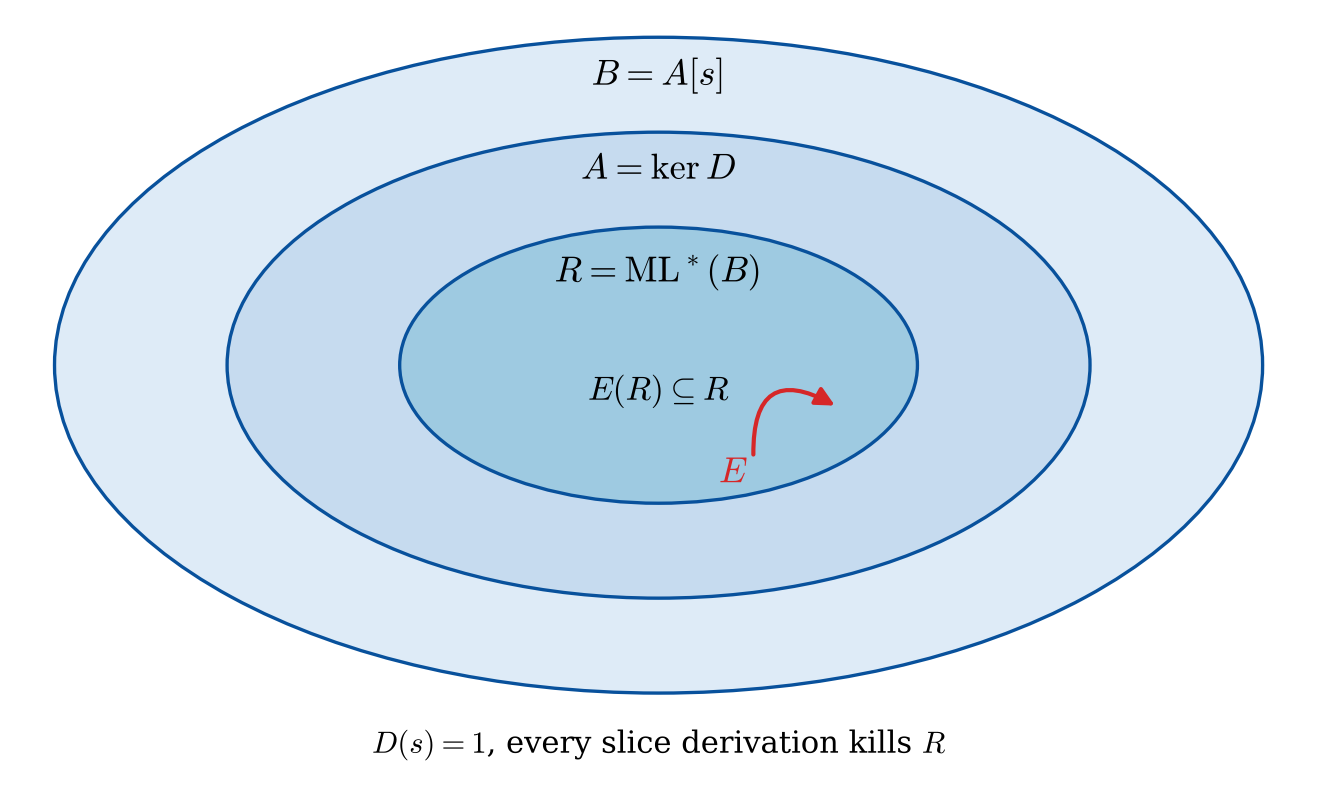
\includegraphics[width=0.62\textwidth]{fig_rings.png}
\caption{The rings in the proofs. A slice derivation $D$ writes $B$ as $A[s]$ with $A=\ker D$, and $R=\MLs(B)$ lies in every such $A$. By Proposition~\ref{prop:stable} an arbitrary locally nilpotent derivation $E$ maps $R$ into itself, even when $E$ moves $A$.}
\label{fig:rings}
\end{figure}

The following extension lemma is \cite[Lemma~3.1(i)]{DG21}; we recall the proof, which we also need for non-affine rings.

\begin{lemma}\label{lem:extend}
Let $D\in\LNDs(B)$ and $A=\ker D$. Then $R\subseteq\ML(A)$.
\end{lemma}

\begin{proof}
By Lemma~\ref{lem:slice}, $B=A[s]$ is a polynomial ring and $D=d/ds$. Let $\delta\in\LND(A)$ and define $\tilde\delta$ on $A[s]$ coefficientwise, $\tilde\delta(\sum_i a_is^i)=\sum_i\delta(a_i)s^i$. It is a $k$-derivation, since $\delta$ is one on $A$ and $\tilde\delta(s)=0$. It is locally nilpotent, because $\tilde\delta^m(\sum_ia_is^i)=\sum_i\delta^m(a_i)s^i$ and only finitely many $a_i$ occur. It commutes with $D$, since for $a\in A$
\[
\tilde\delta D(as^i)=\tilde\delta(ia\,s^{i-1})=i\,\delta(a)s^{i-1}=D\bigl(\delta(a)s^i\bigr)=D\tilde\delta(as^i).
\]
By Lemma~\ref{lem:commuting}, $E=\tilde\delta+D$ is locally nilpotent, and $E(s)=0+1=1$, so $E\in\LNDs(B)$. For $a\in A$ we have $E(a)=\delta(a)$, so $\ker E\cap A=\ker\delta$. Since $R\subseteq\ker D=A$ and $R\subseteq\ker E$, we get $R\subseteq\ker\delta$. This holds for every $\delta\in\LND(A)$, so $R\subseteq\ML(A)$.
\end{proof}

\begin{remark}\label{rem:group}
Lemma~\ref{lem:aut} and Proposition~\ref{prop:stable} say that $R$ is stable under the whole automorphism group of $B$ and under every locally nilpotent derivation, although it is defined by a smaller family. The ring $\ML(B)$ is the ring of invariants of the subgroup of $\Aut(B)$ generated by all the groups $\{\exp(tD):t\in k\}$, and $R$ is the ring of invariants of the subgroup generated by those with $D\in\LNDs(B)$; the second subgroup is normal in the first. Over an algebraically closed field Gaifullin and Shafarevich show that the two subgroups have the same general orbits \cite{GS24}. Group actions and the structures they preserve in other geometric settings are studied in \cite{Bha22a,Bha22b,BSN26}.
\end{remark}

\section{Proofs of the theorems}\label{sec:proofs}

\begin{proof}[Proof of Theorem~\ref{thmA}]
We have $\ML(B)\subseteq R$ (Section~\ref{sec:intro}), so it suffices to show that $R\subseteq\ker E$ for every $E\in\LND(B)$. Fix $E$ and let $\varepsilon=E|_R$, which is a locally nilpotent derivation of the domain $R$ by Proposition~\ref{prop:stable}. Suppose, to reach a contradiction, that $\varepsilon\neq0$, and let $K=\ker\varepsilon\subseteq R$.

By Lemma~\ref{lem:localslice} there is $g\in R$ with $c=\varepsilon(g)\neq0$ and $\varepsilon(c)=0$, and $g$ is not algebraic over $K$. We claim that every element of $K$ is algebraic over $k$. Otherwise some $x\in K$ is transcendental over $k$; as $g$ is not algebraic over $k[x]\subseteq K$, the elements $x$ and $g$ of $R$ are algebraically independent over $k$, which contradicts $\td{R}\le1$.

So $c\in K$ is a nonzero element algebraic over $k$. Let $\mu(T)=T^m+\lambda_{m-1}T^{m-1}+\dots+\lambda_0\in k[T]$ be a monic polynomial of least degree with $\mu(c)=0$. If $\lambda_0=0$, then $c\cdot(c^{m-1}+\lambda_{m-1}c^{m-2}+\dots+\lambda_1)=0$ with $c\neq0$ in a domain, which contradicts the minimality of $m$. Hence $\lambda_0\neq0$ and
\[
c^{-1}=-\lambda_0^{-1}\bigl(c^{m-1}+\lambda_{m-1}c^{m-2}+\dots+\lambda_1\bigr)\in k[c]\subseteq K .
\]
Put $s=c^{-1}g\in R\subseteq B$. Since $c^{-1}\in K$, we have $E(c^{-1})=\varepsilon(c^{-1})=0$, and therefore
\[
E(s)=E(c^{-1})\,g+c^{-1}E(g)=c^{-1}c=1 .
\]
Thus $s$ is a slice of $E$, so $E\in\LNDs(B)$, and by the definition of $R$ we get $R\subseteq\ker E$, that is, $\varepsilon=0$. This contradiction shows $\varepsilon=0$, so $R\subseteq\ker E$.
\end{proof}

The argument shows a little more: if $E\in\LND(B)$ does not kill $\MLs(B)$, then $\ker(E|_{\MLs(B)})$ contains an element transcendental over $k$.\footnote{When $\td{\MLs(B)}=0$ the theorem is also immediate from Lemma~\ref{lem:algclosed}: every element of $\MLs(B)$ is then algebraic over $k$, hence killed by every derivation of $B$.} The step that fails in general is the inversion of $c$: for $\td{\MLs(B)}\ge2$ the element $c=\varepsilon(g)$ may be a non-unit of $K$, and $c^{-1}g$ is then not in $B$.

\begin{proof}[Proof of Theorem~\ref{thmB}]
Since $\td{R}=n-1<n=\td{B}$, we have $R\neq B$, so $\LNDs(B)\neq\emptyset$. Fix $D\in\LNDs(B)$ with slice $s$ and put $A=\ker D$. By Lemma~\ref{lem:slice}, $B=A[s]=A^{[1]}$ and $\td{A}=n-1$.

\emph{Step 1: $R=A$.} We have $R\subseteq A$. Choose $x_1,\dots,x_{n-1}\in R$ algebraically independent over $k$; this is possible because $\Frac(R)$ is generated by $R$. Let $a\in A$. If $a$ were not algebraic over $k[x_1,\dots,x_{n-1}]$, the $n$ elements $x_1,\dots,x_{n-1},a$ of $A$ would be algebraically independent, against $\td{A}=n-1$. So $a$ is algebraic over $R$, and $a\in R$ because $R$ is algebraically closed in $B$ (Section~\ref{sec:stable}). Hence $A=R$, and $B=R^{[1]}$.

\emph{Step 2: $R$ is rigid.} By Lemma~\ref{lem:extend} and Step 1, $R\subseteq\ML(A)=\ML(R)$. So every $\delta\in\LND(R)$ vanishes on $R$, that is, $\LND(R)=\{0\}$.

\emph{Step 3: $\ML(B)=R$.} Let $E\in\LND(B)$. By Proposition~\ref{prop:stable}, $E|_R\in\LND(R)=\{0\}$, so $R\subseteq\ker E$. Hence $R\subseteq\ML(B)\subseteq R$.

\emph{Step 4: $\ker E=R$ for every nonzero $E\in\LND(B)$.} By Step 3, $R\subseteq\ker E$, and by Lemma~\ref{lem:localslice}, $\td{\ker E}\le n-1=\td R$. As in Step 1, every element of $\ker E$ is algebraic over $R$ and hence lies in $R$.
\end{proof}

Step 4 says that $B$ is semi-rigid: all nonzero locally nilpotent derivations have the same kernel.

\begin{proof}[Proof of Theorem~\ref{thmC}]
Let $n=\td{B}$. Fix $D\in\LNDs(B)$ with slice $s$ and $A=\ker D$. Since $s$ is transcendental over $k$ by Lemma~\ref{lem:slice}, $n\ge1$, and $\td{A}=n-1\le2$. As $R\subseteq A$, $\td{R}\le n-1$. If $\td{R}\le1$, Theorem~\ref{thmA} applies. The only remaining case is $n=3$ and $\td{R}=2=n-1$, where Theorem~\ref{thmB} applies.
\end{proof}

\begin{proof}[Proof of Corollary~\ref{corD}]
Let $\td{B}=n$, $\ML(B)=k$ and $k\neq R\neq B$. Since $R\neq B$, $\LNDs(B)\neq\emptyset$ and $\td{R}\le n-1$ by Lemma~\ref{lem:slice}. If $\td{R}\le1$ or $\td{R}=n-1$, Theorems~\ref{thmA} and~\ref{thmB} give $R=\ML(B)=k$, which is excluded. Hence $2\le\td{R}\le n-2$. For $n=3$ this range is empty, and since $\td{R}=1$ forces $R\neq k$ and $R\neq B$, no three-dimensional $B$ has $\ML(B)=k$ and $\td{R}=1$.

For the equivalence, let $\td{B}=3$. If (III) holds, that is $\ML(B)=k$ and $R\neq B$, the case $R\neq k$ has just been excluded, so $R=k$, which is (II). If (II) holds, then $R=k\neq B$ because $\td{B}=3$, and $k\subseteq\ML(B)\subseteq R=k$, which is (III).
\end{proof}

\begin{remark}
The implication (III)$\Rightarrow$(I) of \cite{DG21} is false without its hypotheses: for $k=\RR$ the ring $B=\RR[X,Y,Z]/(XY-Z^2-1)\,[T]$ satisfies $\MLs(B)=\RR$ but is not $\RR^{[3]}$ \cite{DG21}. Corollary~\ref{corD} shows that the failure happens only between (I) and the other two conditions.
\end{remark}

\section{Examples over the real numbers}\label{sec:examples}

The examples in this section show that $\ML$ and $\MLs$ do not commute with extension of the base field, so that results over $\CC$ cannot simply be descended to $\RR$. They also show that the hypotheses of Theorems~\ref{thmA} and~\ref{thmB} occur for rings that are not polynomial rings over $k$.

Let $S=\RR[x,y,z]=\RR[X,Y,Z]/(X^2+Y^2+Z^2-1)$ be the coordinate ring of the real two-sphere, and $S_\CC=S\otimes_\RR\CC$. The polynomial $X^2+Y^2+Z^2-1$ is irreducible over $\CC$, so $S$ and $S_\CC$ are domains of transcendence degree two.\footnote{If it factored into two linear polynomials, its homogenisation $X^2+Y^2+Z^2-W^2$ would be a product of two linear forms; but a product of two linear forms is a quadratic form of rank at most two, and this one has rank four. The transcendence degree is two because $x,y$ are algebraically independent (no nonzero polynomial in $X,Y$ alone lies in the ideal) and $z$ is algebraic over them.}

\begin{proposition}\label{prop:sphere}
\begin{enumerate}
\item[(a)] $S$ is rigid over $\RR$, so $\ML(S)=\MLs(S)=S$.
\item[(b)] $\ML(S[T])=\MLs(S[T])=S$, which has transcendence degree two over $\RR$.
\item[(c)] $\ML(S_\CC)=\CC$, and $\ML(S_\CC[T])=\MLs(S_\CC[T])=\CC$.
\end{enumerate}
\end{proposition}

\begin{figure}[H]
\centering
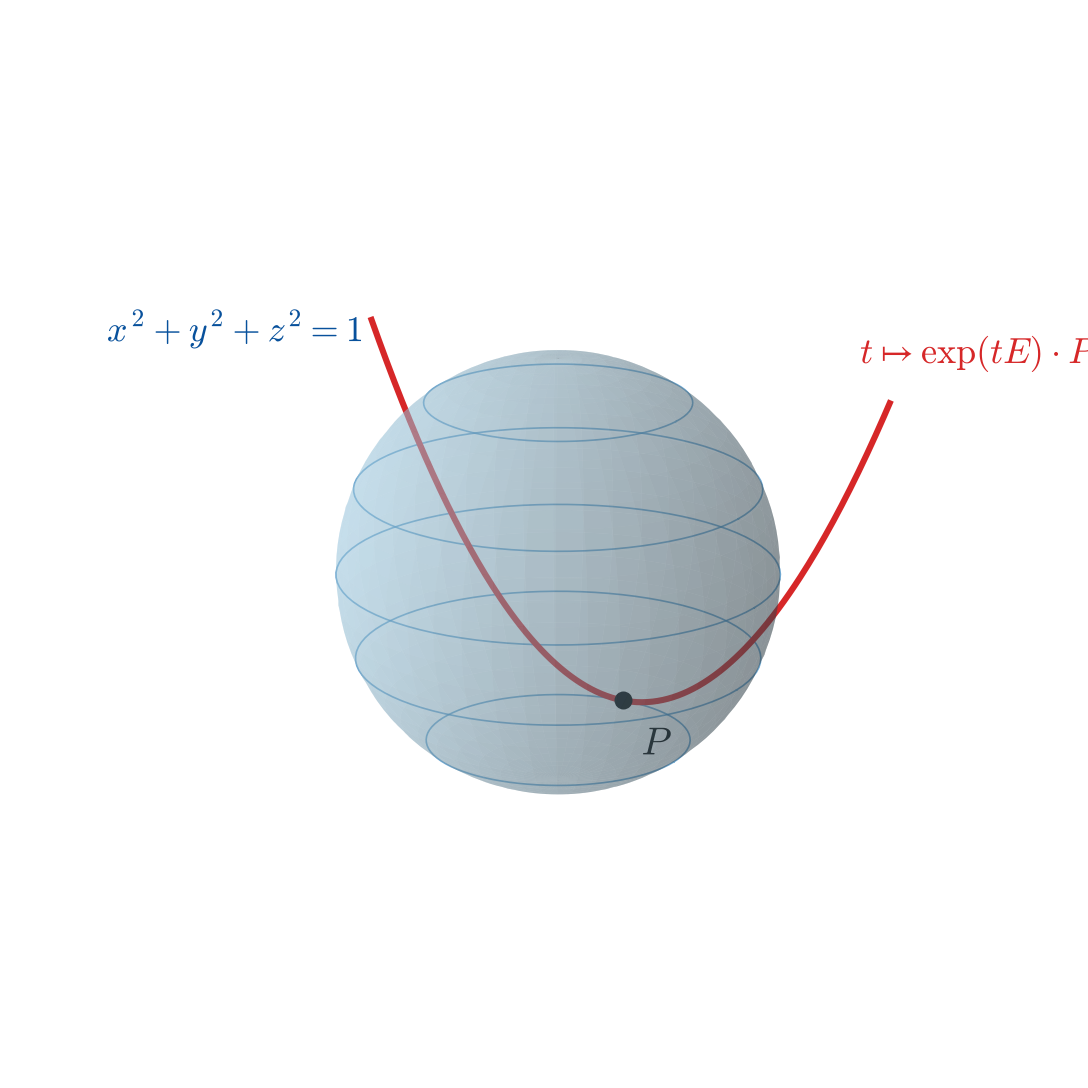
\includegraphics[width=0.46\textwidth]{fig_sphere.png}
\caption{The proof of Proposition~\ref{prop:sphere}(a). For a real point $P$ the orbit $t\mapsto\exp(tE)\cdot P$ is a polynomial curve which must stay on the sphere; a nonconstant real polynomial curve is unbounded, as drawn, so the orbit is a single point.}
\label{fig:sphere}
\end{figure}

\begin{proof}
(a) A point $P=(p_1,p_2,p_3)\in\RR^3$ with $p_1^2+p_2^2+p_3^2=1$ defines an $\RR$-algebra homomorphism $\mathrm{ev}_P\colon S\to\RR$. Let $E\in\LND(S)$. For $f\in S$ the function $t\mapsto\mathrm{ev}_P(\exp(tE)f)=\sum_i t^i\,\mathrm{ev}_P(E^if)/i!$ is a real polynomial in $t$. Let $X(t),Y(t),Z(t)$ be these polynomials for $f=x,y,z$. Since $\exp(tE)$ is an algebra homomorphism (Lemma~\ref{lem:exp}),
\[
X(t)^2+Y(t)^2+Z(t)^2=\mathrm{ev}_P\bigl(\exp(tE)(x^2+y^2+z^2)\bigr)=\mathrm{ev}_P(1)=1
\]
for all $t\in\RR$. If the largest of the degrees of $X,Y,Z$ were $d\ge1$, the coefficient of $t^{2d}$ on the left would be the sum of the squares of the leading coefficients of those polynomials of degree $d$, which is positive. So $X,Y,Z$ are constant, and comparing the coefficients of $t$ gives $\mathrm{ev}_P(E x)=\mathrm{ev}_P(E y)=\mathrm{ev}_P(E z)=0$.

Thus $Ex$, $Ey$, $Ez$ vanish at every real point of the sphere. We show that such an element $f\in S$ is zero. Dividing by the monic polynomial $Z^2-(1-X^2-Y^2)$ in $Z$, write $f=a(x,y)+z\,b(x,y)$ with $a,b\in\RR[X,Y]$. For $(p_1,p_2)$ in the open unit disc, both $(p_1,p_2,\pm\sqrt{1-p_1^2-p_2^2})$ are real points, so $a(p_1,p_2)\pm r\,b(p_1,p_2)=0$ with $r=\sqrt{1-p_1^2-p_2^2}>0$. Hence $a$ and $b$ vanish on the open disc, so $a=b=0$ as polynomials, and $f=0$. Therefore $E$ kills the generators $x,y,z$, so $E=0$. Since $\LND(S)=\{0\}$, also $\LNDs(S)=\emptyset$ and $\MLs(S)=S$.

(b) The derivative $\partial_T$ has the slice $T$ and kernel $S$, so $\ML(S[T])\subseteq\MLs(S[T])\subseteq S$. Conversely, let $E\in\LND(S[T])$. The argument of (a), applied at the real points $(P,\tau)$ with $P$ on the sphere and $\tau\in\RR$, shows that $Ex,Ey,Ez$ vanish at all of them. An element $\sum_jf_jT^j$ of $S[T]$ ($f_j\in S$) vanishing at all these points has $f_j(P)=0$ for all $j$ and all $P$, since a real polynomial in $\tau$ with infinitely many roots is zero; so each $f_j=0$ by (a). Hence $E$ kills $S$, and $S\subseteq\ML(S[T])$. The same conclusion follows from Theorem~\ref{thmB}, once one knows that $\td{\MLs(S[T])}=2$.

(c) Put $u=x+iy$ and $v=x-iy$ in $S_\CC$. Then $uv=x^2+y^2=1-z^2$, and $S_\CC=\CC[u,v,z]$ with the single relation $uv+z^2-1=0$. Define a $\CC$-derivation $D_1$ by $D_1(u)=0$, $D_1(z)=u$, $D_1(v)=-2z$. It is well defined, since $D_1(uv+z^2-1)=u(-2z)+2zu=0$. It is locally nilpotent by Lemma~\ref{lem:generators}, since $D_1^2(z)=0$ and $D_1^3(v)=-2D_1^2(z)=0$. Symmetrically, $D_2(v)=0$, $D_2(z)=v$, $D_2(u)=-2z$ defines $D_2\in\LND(S_\CC)$.

The localisation $S_\CC[u^{-1}]$ equals $\CC[u^{\pm1},z]$, because $v=(1-z^2)/u$. Here $u$ and $z$ are algebraically independent, since they generate a field of transcendence degree two. Extend $D_1$ to $S_\CC[u^{-1}]$ by $D_1(b/u^m)=D_1(b)/u^m$, which is possible as $D_1(u)=0$. On $\CC[u^{\pm1}][z]$ it acts as $u\,\partial/\partial z$, whose kernel is $\CC[u^{\pm1}]$. Hence $\ker D_1\subseteq\CC(u)$, and in the same way $\ker D_2\subseteq\CC(v)$. The elements $u,v$ are algebraically independent, because $z$ is algebraic over $\CC(u,v)$ through $z^2=1-uv$. In the field $\CC(u,v)$ one has $\CC(u)\cap\CC(v)=\CC$.\footnote{If $p(u)/q(u)=r(v)/s(v)$ with coprime $p,q$ and coprime $r,s$, then $p(u)s(v)=q(u)r(v)$ in the polynomial ring $\CC[u,v]$. Since $q(u)$ is coprime to $p(u)$, it divides $s(v)$, so $q$ is constant; likewise $s$ is constant, and then $p(u)$ is a constant multiple of $r(v)$, so both are constant.} So $\ML(S_\CC)\subseteq\ker D_1\cap\ker D_2=\CC$.

Extend $D_1$ and $D_2$ to $S_\CC[T]$ by $D_i(T)=0$. Each commutes with $\partial_T$, so $D_i+\partial_T$ is locally nilpotent by Lemma~\ref{lem:commuting}, and it has the slice $T$. On $S_\CC$ it agrees with $D_i$. Using also $\partial_T$, whose kernel is $S_\CC$,
\[
\MLs(S_\CC[T])\subseteq S_\CC\cap\ker(D_1+\partial_T)\cap\ker(D_2+\partial_T)=\ker D_1\cap\ker D_2=\CC .
\]
Since $\ML\subseteq\MLs$ and both contain $\CC$, both equal $\CC$.
\end{proof}

So the real ring $S[T]$ has $\ML=\MLs=S$, of transcendence degree two, while after extension to $\CC$ both invariants become $\CC$. The equality $\ML=\MLs$ over $\CC$, which is part of \cite[Theorem~1]{GS24}, therefore carries no information about the two real invariants: both change. The hyperboloid used by Dasgupta and Gupta behaves in the opposite way, with $\MLs$ already trivial over $\RR$ \cite{DG21}.

\begin{example}\label{ex:circle}
Let $C=\RR[x,y]/(x^2+y^2-1)$ be the coordinate ring of the real circle and $B=C[T_1,T_2]$. The argument of Proposition~\ref{prop:sphere}(a), with $X(t)^2+Y(t)^2=1$, shows that $C$ is rigid and that every locally nilpotent derivation of $B$ kills $C$. The derivations $\partial_{T_1}$ and $\partial_{T_2}$ have slices and $\ker\partial_{T_1}\cap\ker\partial_{T_2}=C$. Hence $\ML(B)=\MLs(B)=C$, of transcendence degree one, as Theorem~\ref{thmA} predicts.
\end{example}

\section{Remarks on the open cases}\label{sec:open}

\subsection*{Higher dimension}
Let $\td{B}=n\ge4$ and $2\le\td{\MLs(B)}\le n-2$. The proof of Theorem~\ref{thmA} still gives the following: if $E\in\LND(B)$ does not kill $R=\MLs(B)$, then $K=\ker(E|_R)$ contains elements transcendental over $k$, and no local slice $g\in R$ of $E|_R$ has $E(g)$ invertible in $R$. Lemma~\ref{lem:extend} gives $R\subseteq\ML(A)$ for every slice kernel $A$. For $n=4$ and $\td R=2$ this says that $R$ is a two-dimensional subring of the three-dimensional ring $A$ killed by every locally nilpotent derivation of $A$. Over an algebraically closed field the equality $\ML(B)=\MLs(B)$ is known in all these cases \cite{GS24}. We do not know whether it holds over $\RR$ or $\QQ$, and the methods above do not decide it.

\subsection*{Positive characteristic}
In characteristic $p>0$ locally nilpotent derivations are replaced by exponential maps, and $\ML$ and $\MLs$ are defined in the same way. Sai Krishna asked whether $\MLs(B)\neq B$ implies $\MLs(B)=\ML(B)$ for affine domains over algebraically closed fields of arbitrary characteristic, and answered it in some cases \cite{Sai24}. Our proofs use characteristic zero in Lemma~\ref{lem:algclosed}, where the derivative $P'$ must be nonzero, and in the division by $i!$. They do not apply to that question.

\section*{Declarations}

\noindent\textbf{Data availability.} No data were generated or analysed. The \LaTeX\ source of this paper and the script that draws its figures are archived at \href{https://doi.org/\zenodoCodeDOI}{doi:\zenodoCodeDOI}.

\smallskip\noindent\textbf{Funding.} The author received no funding for this work.

\smallskip\noindent\textbf{Conflict of interest.} The author declares no conflict of interest.

\smallskip\noindent\textbf{Ethics statement.} This work involves no human or animal subjects.

\begin{thebibliography}{99}

\bibitem{AFKKZ13} I.~Arzhantsev, H.~Flenner, S.~Kaliman, F.~Kutzschebauch and M.~Zaidenberg, Flexible varieties and automorphism groups, \emph{Duke Math. J.} \textbf{162} (2013), no.~4, 767--823. doi:10.1215/00127094-2080132.

\bibitem{Bha22a} D.~Bhattacharjee, Non-commutativity over canonical suspension $\eta$ for genus $g\ge1$ in hypercomplex structures for potential $\rho\phi$, \emph{Asian Res. J. Math.} \textbf{18} (2022), no.~11, 332--341. doi:10.9734/arjom/2022/v18i11607.

\bibitem{Bha22b} D.~Bhattacharjee, Establishing equivariant class $[O]$ for hyperbolic groups, \emph{Asian Res. J. Math.} \textbf{18} (2022), no.~11, 362--369. doi:10.9734/arjom/2022/v18i11615.

\bibitem{BSN26} D.~Bhattacharjee, S.~Singha Roy and P.~Nandi, Hodge--toric geometry beyond CY20, \emph{Int. J. Prof. Stud.} \textbf{21} (2026), no.~1. doi:10.37648/ijps.v21i01.019.

\bibitem{CML05} A.~J.~Crachiola and L.~Makar-Limanov, On the rigidity of small domains, \emph{J. Algebra} \textbf{284} (2005), no.~1, 1--12. doi:10.1016/j.jalgebra.2004.09.015.

\bibitem{DG21} N.~Dasgupta and N.~Gupta, An algebraic characterization of the affine three space, \emph{J. Commut. Algebra} \textbf{13} (2021), no.~3, 333--345. doi:10.1216/jca.2021.13.333.

\bibitem{Dub09} A.~Dubouloz, The cylinder over the Koras--Russell cubic threefold has a trivial Makar-Limanov invariant, \emph{Transform. Groups} \textbf{14} (2009), no.~3, 531--539. doi:10.1007/s00031-009-9051-3.

\bibitem{Fre17} G.~Freudenburg, \emph{Algebraic Theory of Locally Nilpotent Derivations}, 2nd ed., Encyclopaedia Math. Sci. \textbf{136}, Springer, Berlin, 2017. doi:10.1007/978-3-662-55350-3.

\bibitem{GS24} S.~Gaifullin and A.~Shafarevich, Modified Makar-Limanov and Derksen invariants, \emph{J. Pure Appl. Algebra} \textbf{228} (2024), no.~6, 107616. doi:10.1016/j.jpaa.2024.107616.

\bibitem{Gup14a} N.~Gupta, On the cancellation problem for the affine space $\mathbb A^3$ in characteristic $p$, \emph{Invent. Math.} \textbf{195} (2014), no.~1, 279--288. doi:10.1007/s00222-013-0455-2.

\bibitem{Gup14b} N.~Gupta, On Zariski's cancellation problem in positive characteristic, \emph{Adv. Math.} \textbf{264} (2014), 296--307. doi:10.1016/j.aim.2014.07.012.

\bibitem{ML96} L.~Makar-Limanov, On the hypersurface $x+x^2y+z^2+t^3=0$ in $\mathbb C^4$ or a $\mathbb C^3$-like threefold which is not $\mathbb C^3$, \emph{Israel J. Math.} \textbf{96} (1996), no.~2, 419--429. doi:10.1007/BF02937314.

\bibitem{Sai24} P.~M.~S.~Sai Krishna, An algebraic characterization of the affine three space in arbitrary characteristic, \emph{J. Commut. Algebra} \textbf{16} (2024), no.~3, 293--303. doi:10.1216/jca.2024.16.293.

\end{thebibliography}

\end{document}
